
\documentclass[a4paper,12pt]{article}

\usepackage{graphicx} % Required for inserting images
\usepackage{amsmath,amssymb,amsfonts}
\usepackage{subcaption}
% -----------------------
% Package Imports
% -----------------------

% Set page margins
\usepackage[a4paper, top=1in, bottom=0.8in, left=1.1in, right=0.8in]{geometry}

% Use Times New Roman font
\usepackage{times}

% Add page numbering
\pagestyle{plain}

% Enable graphics inclusion
\usepackage{graphicx}
\usepackage{float}
% Enable code listings
\usepackage{listings}
\usepackage{xcolor} % For customizing code colors
\setlength{\parindent}{0pt}


\begin{document}
	
	
	
	\section{Experiment No. 1}
	
	\section{Experiment Title }
	Introduction to MICROWIND 3.0\\ Design and Analyze nMOS and pMOS layout ensuring proper DRC.
	% Objective Section
	\section{Objective}
	The main objectives of this report are:
	\begin{itemize}
		\item To introduce the use of Microwind 3.0 software for designing and simulating MOSFET transistors (nMOS and pMOS)
		\item To explain the theory and working process of nMOS and pMOS transistors.
		\item To demonstrate the step-by-step fabrication process of nMOS and pMOS transistors using diffusion layers, polysilicon, and the MOS generator tool in Microwind ensuring proper DRC.
	\end{itemize}
	% Theory Section
	\section{Theory}
	\textbf{MICROWIND 3.0} is a specialized software tool designed for the simulation and design of microelectronic circuits at the layout level. It allows users to design, simulate, and analyze semiconductor components like MOSFETs (nMOS and pMOS), digital circuits, and analog circuits by providing a graphical interface that bridges the gap between circuit design and physical layout.
	
	\subsection{Microwind 3.0 Interface Overview}
	
	\begin{figure}[h]
		\centering
		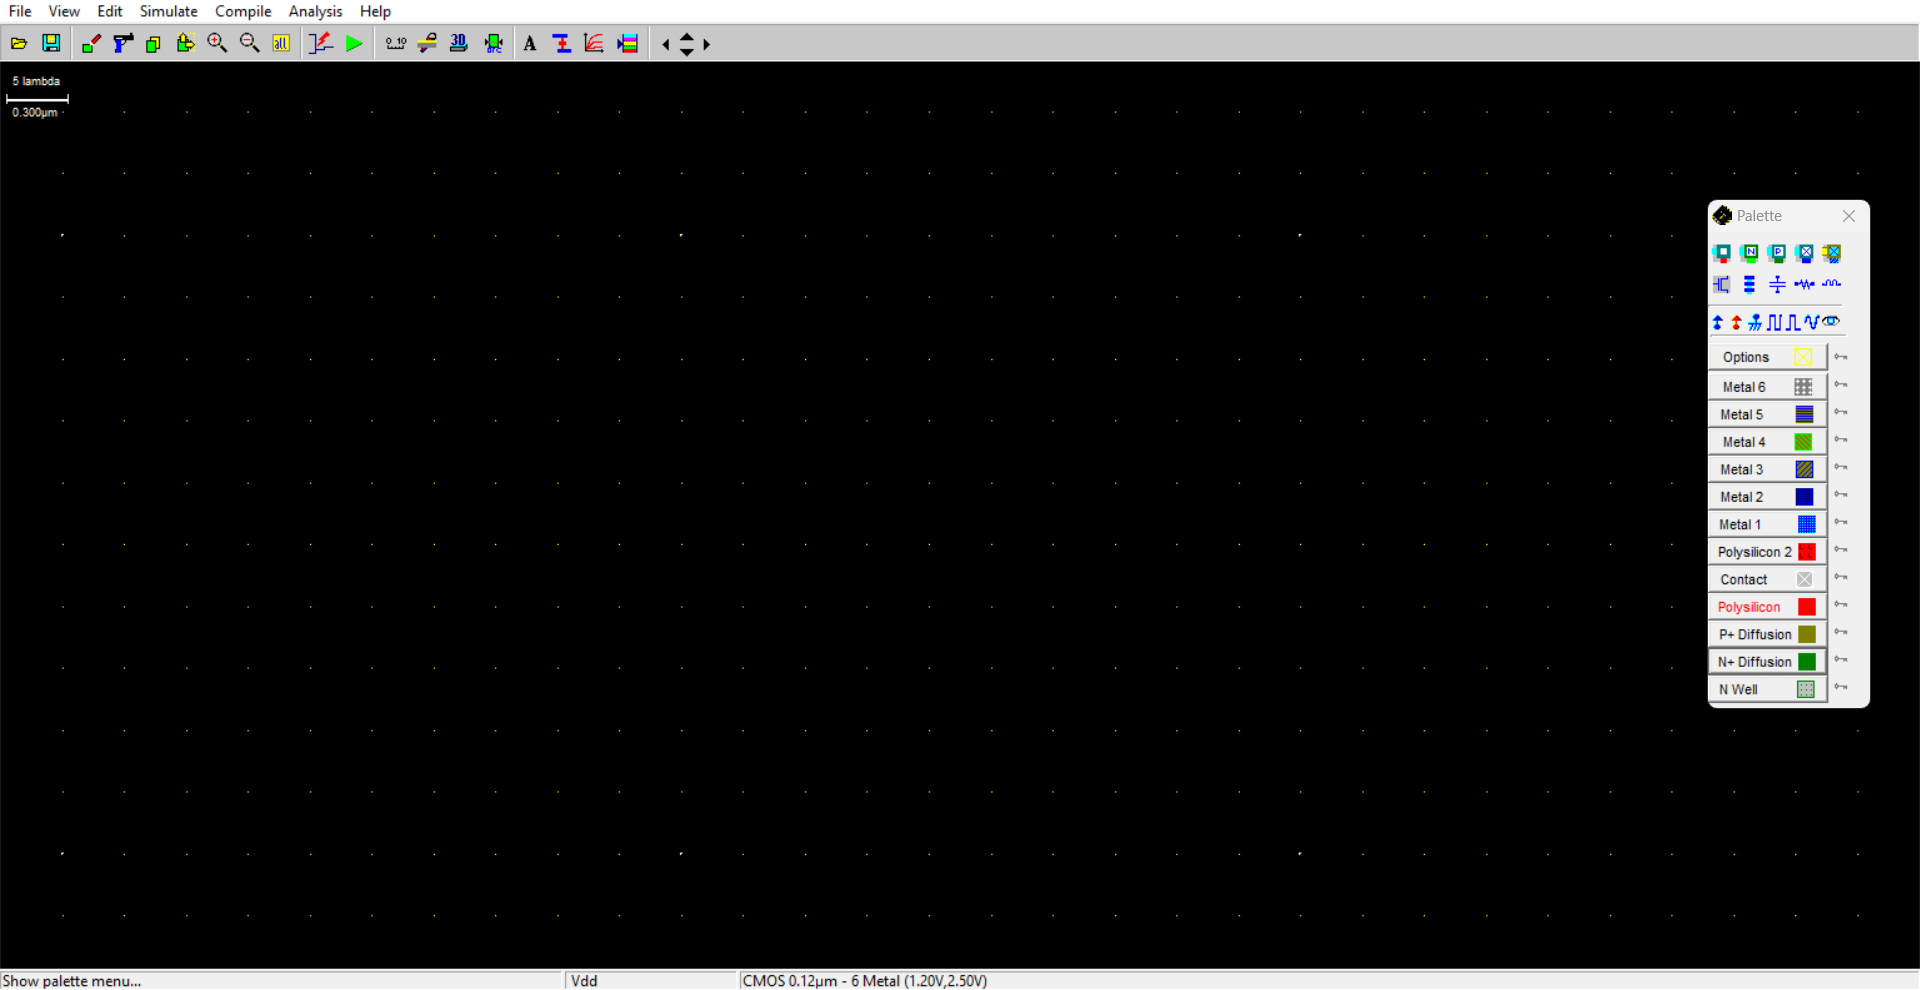
\includegraphics[width=1\linewidth]{Images/microwind/window}
		\caption{Openning Window}
		\label{fig:window}
	\end{figure}
	\newpage
	The Microwind 3.0 interface consists of several key components, each serving a specific purpose in circuit design and simulation. The main parts of the interface include:
	
	\begin{itemize}
		\item Menu Bar
		\item Toolbar
		\item Palette
		\item Simulation Window
		\item DRC (Design Rule Check)
	\end{itemize}
	
	\subsubsection{Menu Bar}
	The menu bar provides access to a wide range of functionalities, organized into several categories:
	
	\begin{figure}[h]
		\centering
		
\includegraphics[width=.7\linewidth]{Images/microwind/menubar}
		\caption{Menu Bar}
		\label{fig:menubar}
	\end{figure}
	
	\begin{itemize}
		\item \textbf{File Menu ,View Menu \& Edit Menu :}
		\begin{figure}[H]
			\centering
			\begin{subfigure}[t]{0.49\textwidth}
				\centering
				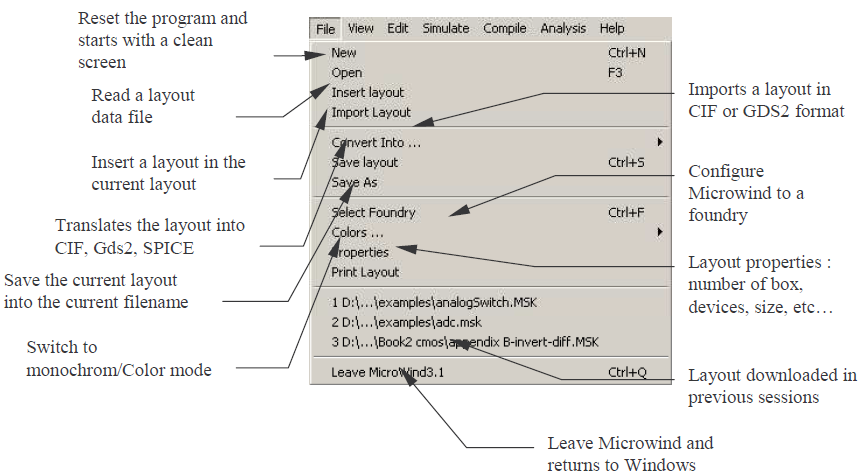
\includegraphics[width=1\textwidth , height=.24\textheight]{Images/microwind/filemenu.png}
				\caption{File Menu}
				\label{fig:3-a}
			\end{subfigure}
			\hfill
			\begin{subfigure}[t]{0.49\textwidth}
				\centering
				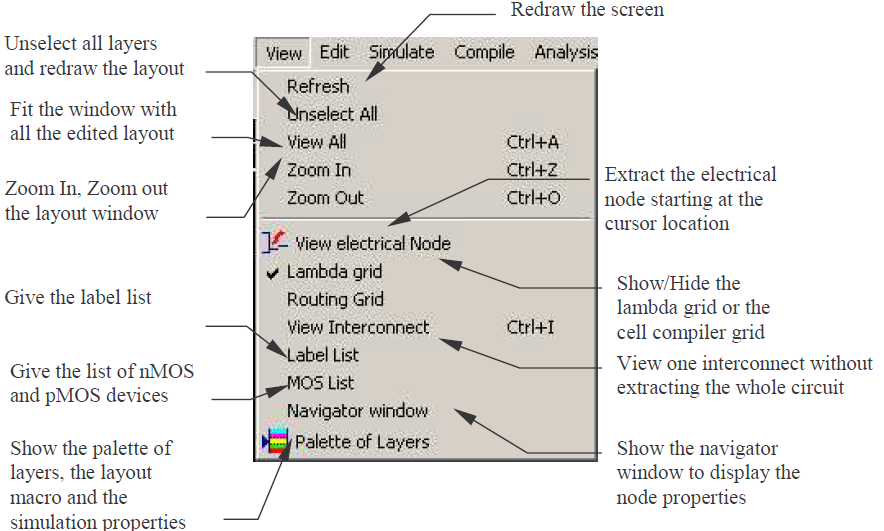
\includegraphics[width=1\textwidth , height=.24\textheight]{Images/microwind/viewmenu.png}
				\caption{View Menu}
				\label{fig:3-b}
			\end{subfigure}
			\begin{subfigure}[t]{0.49\textwidth}
				\centering
				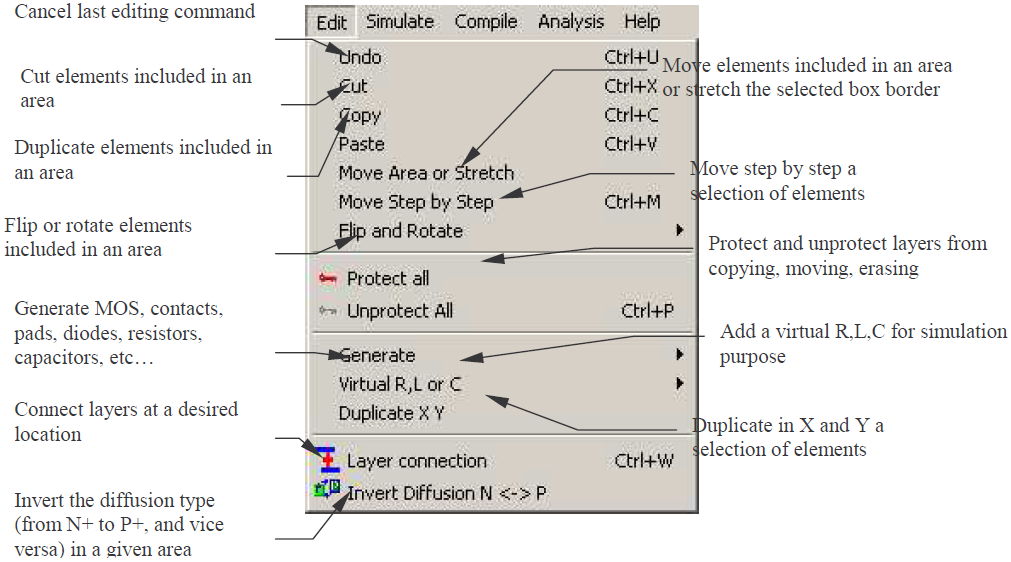
\includegraphics[width=1\textwidth , height=.24\textheight]{Images/microwind/editmenu.png}
				\caption{Edit Menu}
				\label{fig:3-c}
			\end{subfigure}
			\caption{File Menu ,View Menu \& Edit Menu}
		\end{figure}
		
		\newpage
		%%%%%%%%%%%%%%%%%%%%%%%%%%%%%%%%%%%%%%%%%%%%%%%%%%%%%%%%%%%%%%%%%%%%%%%%%%%%%%%%%%%%%
		\item \textbf{Simulate Menu ,Compile Menu \& Analysis Menu :}
		\begin{figure}[H]
			\centering
			\begin{subfigure}[t]{0.5\textwidth}
				\centering
				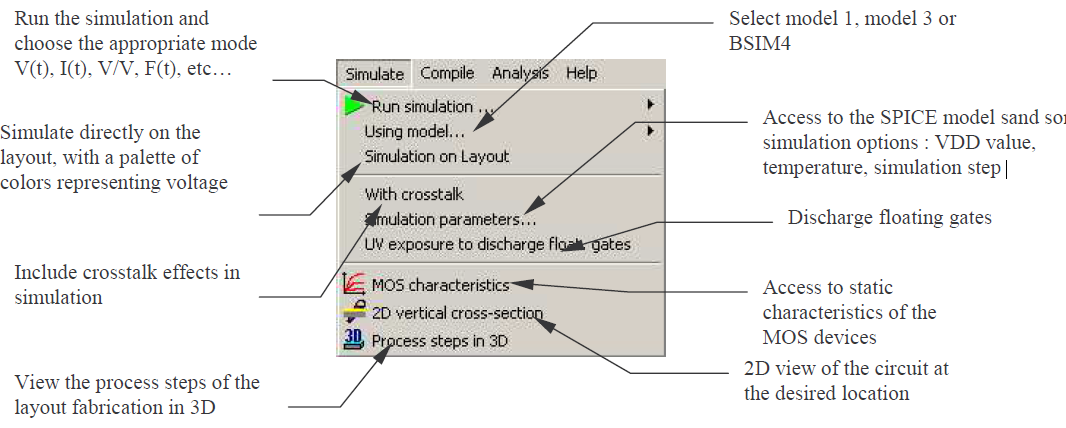
\includegraphics[width=1\textwidth , height=.17\textheight]{Images/microwind/simulatemenu.png}
				\caption{Simulate Menu}
				\label{fig:4-a}
			\end{subfigure}
			\hfill
			\begin{subfigure}[t]{0.49\textwidth}
				\centering
				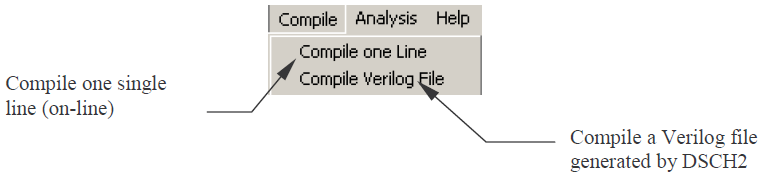
\includegraphics[width=1\textwidth ]{Images/microwind/compilemenu.png}
				\caption{Compile Menu}
				\label{fig:4-b}
			\end{subfigure}
			\begin{subfigure}[t]{0.6\textwidth}
				\centering
				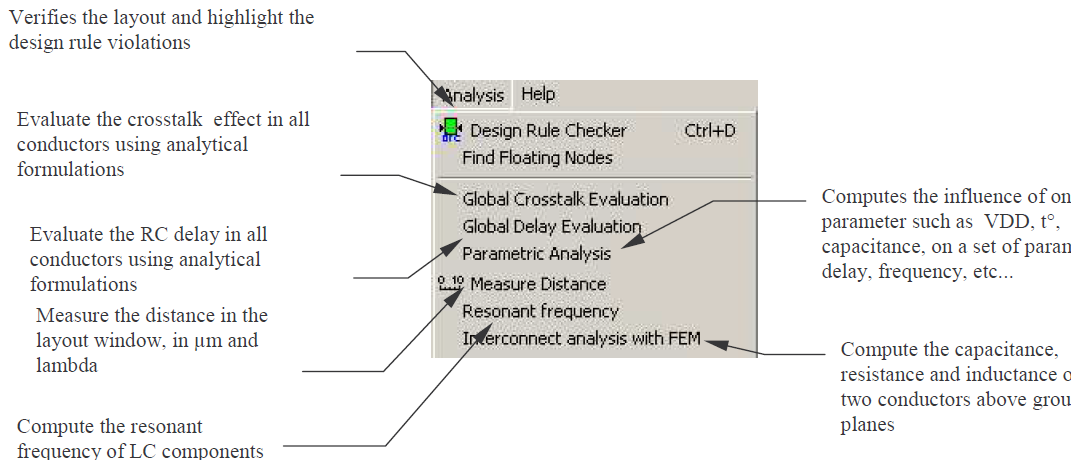
\includegraphics[width=1\textwidth , height=.21\textheight]{Images/microwind/analysismenu2.png}
				\caption{Analysis Menu}
				\label{fig:4-c}
			\end{subfigure}
			\caption{Simulate Menu ,Compile Menu \& Analysis Menu}
			
		\end{figure}
		
	\end{itemize}
	Description about these menus are given below:
	\begin{enumerate}
		
		\item \textbf{File Menu:}
		The File menu allows to create, open, save, and manage design files in Microwind, as well as print layouts.
		\item \textbf{	View Menu:} The View menu offers options to zoom, display gridlines, and toggle visibility of layers or design elements in the layout.
		\item \textbf{Edit Menu:}	 The Edit menu provides tools for copying, pasting, deleting, and modifying elements in the design, such as wires or components.
		\item \textbf{Simulate Menu:}	 The Simulate menu enables running simulations of the circuit to observe signal behavior and performance under various conditions.
		\item \textbf{	Compile Menu:} The Compile menu is used to compile the layout into a netlist, converting the physical design into a file that can be used for simulation.
		\item \textbf{Analysis Menu:}	 The Analysis menu offers tools for analyzing electrical properties, such as signal timing, power consumption, and transistor characteristics.
		
		
	\end{enumerate}
	\newpage
	\subsubsection{Tool Bar}
	\begin{figure}[H]
		\centering
		
\includegraphics[width=1\linewidth]{Images/microwind/toolbar}
		\caption{Tool Bar}
		\label{fig:toolbar}
	\end{figure}
	
	Description about these icons are given below:
	
	\begin{table}[h]
		\caption{Toolbar in Microwind 3.0}
		\centering
		
		\begin{tabular}{c}
			
			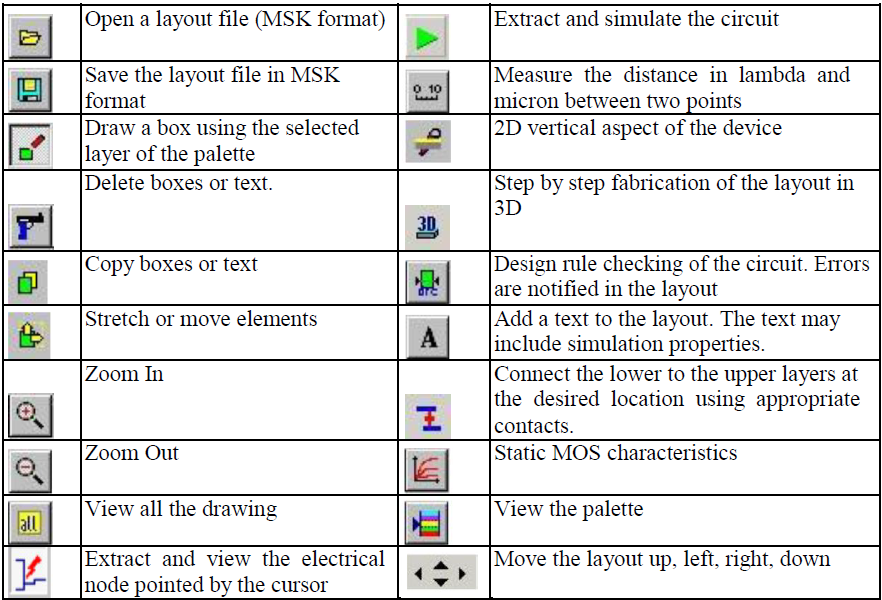
\includegraphics[width=1\linewidth]{Images/microwind/toolbar3} 
			
		\end{tabular}
		
		\label{tab:toolbar}
	\end{table}
	
	\newpage
	
	\subsubsection{Palette}
	The palette contains various tools and options for placing circuit components like transistors, wires, contacts, and vias. Each category is organized based on its function in the layout.
	\begin{figure}[H]
		\centering
		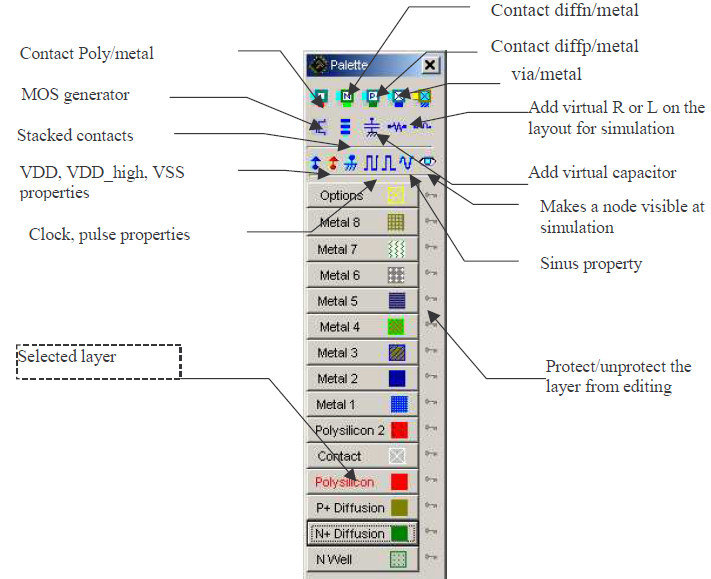
\includegraphics[width=1\linewidth]{Images/microwind/palette}
		\caption{Palette in Microwind 3.0}
		\label{fig:palette}
	\end{figure}
	
	\subsubsection{Simulation Window}
	
	The simulation window shows the results of running an electrical simulation on your layout. This could be in the form of waveforms, timing analysis, or voltage/current plots.
	During simulation, the voltage, current, and logic levels of different nodes in the circuit can be visualized using waveforms. This allows users to verify that the circuit is operating as expected.
	The simulation window also supports timing analysis for digital circuits. Important timing parameters such as delay, rise and fall times, and propagation delays can be measured.
	\begin{figure}[H]
		\centering
		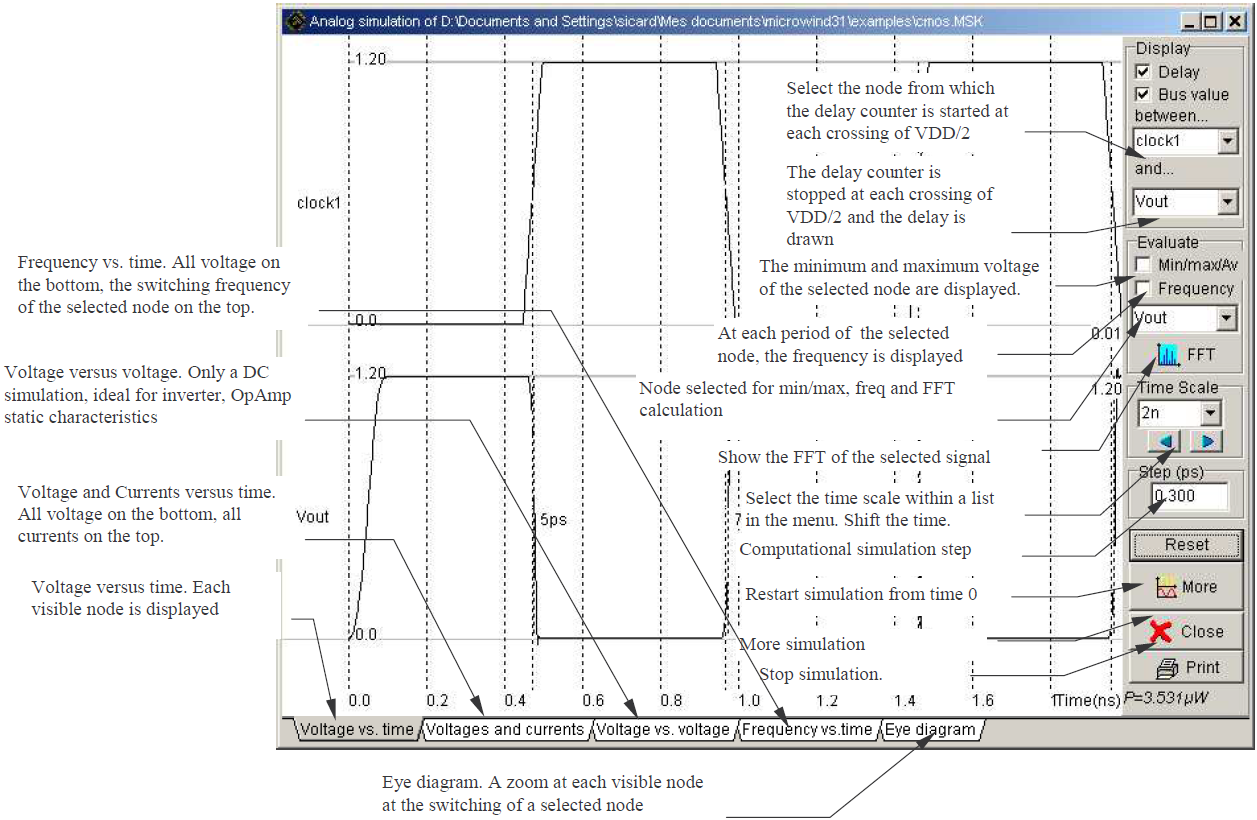
\includegraphics[width=1\linewidth]{Images/microwind/simuwindow}
		\caption{Simulation Window in Microwind 3.0}
		\label{fig:simuwindow}
	\end{figure}
	\subsubsection{DRC (Design Rule Check)}
	Microwind’s layout editor includes a built-in DRC system that alerts users to any violations of the design rules (e.g., minimum distance between components, minimum width for metal layers). This ensures that the layout conforms to the technological requirements for fabrication.
	
	\subsection{Theory of nMOS and pMOS Transistors}
	
	\subsubsection{nMOS Transistor}
	
	The \textbf{nMOS transistor} is a type of MOSFET (Metal-Oxide-Semiconductor Field-Effect Transistor) where the majority charge carriers are electrons. In nMOS, when a positive voltage is applied to the gate terminal, it attracts electrons towards the gate, forming a conductive channel between the source and drain, allowing current to flow from the drain to the source.
	
	The key characteristics of an nMOS transistor include:
	\begin{itemize}
		\item It turns ON when a positive voltage is applied to the gate.
		\item Electrons are the majority carriers in the nMOS.
		\item When the gate voltage is zero or below the threshold voltage, the transistor is OFF, and no current flows.
	\end{itemize}
	
	\subsubsection{pMOS Transistor}
	
	The \textbf{pMOS transistor} is the opposite of nMOS, where the majority charge carriers are holes. When a negative voltage is applied to the gate terminal, it attracts holes, forming a conductive channel, and allows current to flow from the source to the drain.
	
	The key characteristics of a pMOS transistor include:
	\begin{itemize}
		\item It turns ON when a negative voltage is applied to the gate.
		\item Holes are the majority carriers in the pMOS.
		\item When the gate voltage is zero or positive, the transistor is OFF.
	\end{itemize}
	
	\subsubsection{ Strong 0 - Poor 1 and Strong 1 - Poor 0 Concept}
	
	The strength of the 0 and 1 states in nMOS and pMOS transistors comes from their ability to pass or drive voltages effectively. This behavior is related to the nature of the carriers that control the current flow in the transistors—electrons in nMOS and holes in pMOS.
	
	\begin{enumerate}
		\item \textbf{nMOS Transistor:} 
		\begin{enumerate}
			\item \textbf{Strong 0:}
			In an nMOS transistor, when it is ON (the gate voltage is high), it connects the output to ground (0V), meaning it pulls the output low efficiently. Electrons, which are the majority charge carriers in nMOS, are highly mobile and can pull the output to a low voltage (strong 0) quickly and with little resistance.
			\item \textbf{Poor 1: }
			When an nMOS transistor tries to pass a high voltage (logical 1), it does so inefficiently because it connects the output to the power supply $(V_{dd})$ through a pull-up resistor or pMOS. Electrons are not as good at pulling up the voltage to a strong 1 as pMOS transistors. As a result, the output may only reach a slightly higher voltage, but not a full logical high, which is why it's considered a poor 1.
		\end{enumerate}
		\item \textbf{pMOS Transistor:} 
		\begin{enumerate}
			\item \textbf{Strong 1:}
			A pMOS transistor is ON when its gate is at a low voltage (typically 0V). When ON, it connects the output to the power supply $(V_{dd})$ and can pull the output voltage high (logical 1) very effectively. Holes, which are the majority charge carriers in pMOS transistors, can easily move towards the source terminal, enabling a strong high voltage at the output (strong 1).
			\item \textbf{Poor 0: }
			A pMOS transistor does not pass a low voltage (logical 0) very well because holes are less efficient at pulling the output voltage down to 0V. Thus, when a pMOS transistor is used to pass a logical 0, it results in a higher voltage (closer to $V_{dd}$), leading to a poor 0.
		\end{enumerate}
		
	\end{enumerate}
	
	\subsection{Fabrication Process of nMOS and pMOS in Microwind}
	
	\subsubsection{Using Diffusion Layer and Polysilicon}
	
	In Microwind,we can fabricate an nMOS or pMOS transistor using the following steps:
	
	\begin{enumerate}
		\item \textbf{nMOS Transistor:}
		\begin{enumerate}
			\item Draw the \textit{n-diffusion} layer to define the region for the source and drain.
			\item Place the \textit{polysilicon} layer over the diffusion to form the gate terminal.
			\item The intersection of the polysilicon and diffusion layer forms the channel of the transistor.
			\item Add \textit{contacts} to the diffusion regions to form the source and drain terminals.
			\item Complete the circuit by ensuring proper DRC.
		\end{enumerate}
		
		\item \textbf{pMOS Transistor:}
		\begin{enumerate}
			\item Draw the \textit{p-diffusion} layer to define the region for the source and drain.
			\item Place the \textit{polysilicon} layer over the diffusion to form the gate terminal.
			\item The intersection of the polysilicon and diffusion layer forms the channel of the transistor.
			\item Add \textit{contacts} to the diffusion regions to form the source and drain terminals.
			\item Add \textit{n-well} to the whole transistor region of Vdd++(5V).
			\item Complete the circuit by ensuring proper DRC..
		\end{enumerate}
	\end{enumerate}
	
	\subsubsection{Using MOS Generator in Microwind}
	
	Microwind also provides an automatic tool called the \textbf{MOS Generator} to simplify the transistor creation process. Here are the steps to fabricate nMOS and pMOS transistors using the MOS Generator:
	
	\begin{enumerate}
		\item \textbf{nMOS Transistor:}
		\begin{enumerate}
			\item Open the MOS Generator tool.
			\item Select \textit{nMOS} from the options.
			\item Adjust the width and length of the transistor as required.
			\item The MOS Generator automatically generates the necessary diffusion, polysilicon, and contact layers.
		\end{enumerate}
		
		\item \textbf{pMOS Transistor:}
		\begin{enumerate}
			\item Open the MOS Generator tool.
			\item Select \textit{pMOS} from the options.
			\item Adjust the width and length of the transistor as required.
			\item The MOS Generator automatically generates the necessary diffusion, polysilicon, and contact layers.
		\end{enumerate}
	\end{enumerate}
	
	Using the MOS Generator is particularly efficient, as it automates the design of the transistor structure, reducing the time and complexity involved in manual layout.
	
	
	
	
	
	
	\newpage
	\section{Schematic Layout }
	\begin{figure}[H]
		\centering
		
		\begin{subfigure}[t]{0.49\textwidth}
			\centering
			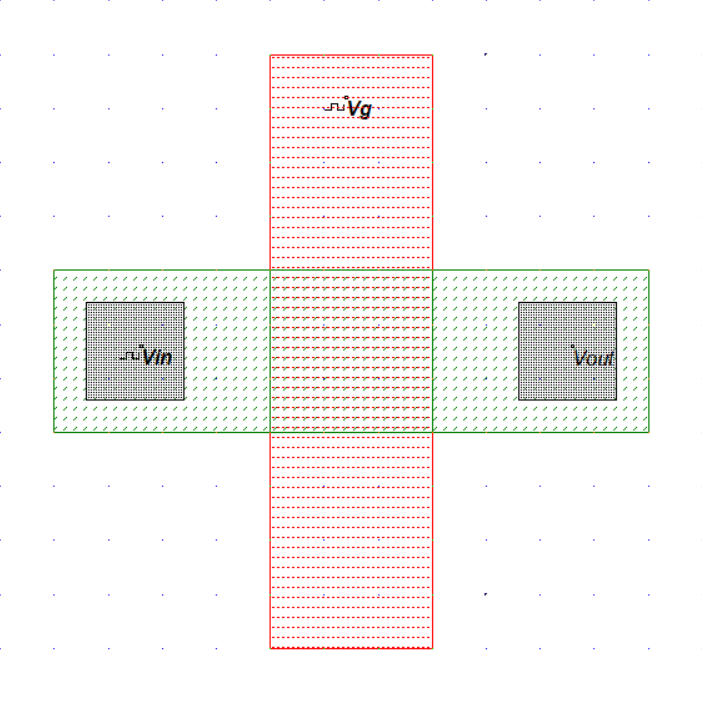
\includegraphics[width=1\textwidth , height=.25\textheight]{Images/nmos/nmos1.png}
			\caption{nMOS}
			\label{fig:3-a}
		\end{subfigure}
		\hfill
		\begin{subfigure}[t]{0.49\textwidth}
			\centering
			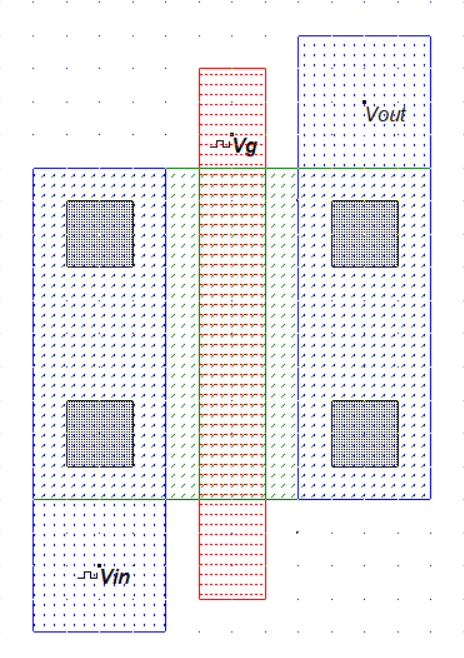
\includegraphics[width=.7\textwidth, height=0.25\textheight]{Images/Builtin nmos/nmos2.png}
			\caption{nMOS (using MOS Generator)}
			\label{fig:3-b}
		\end{subfigure}
		\\[2cm]
		\begin{subfigure}[t]{0.49\textwidth}
			\centering
			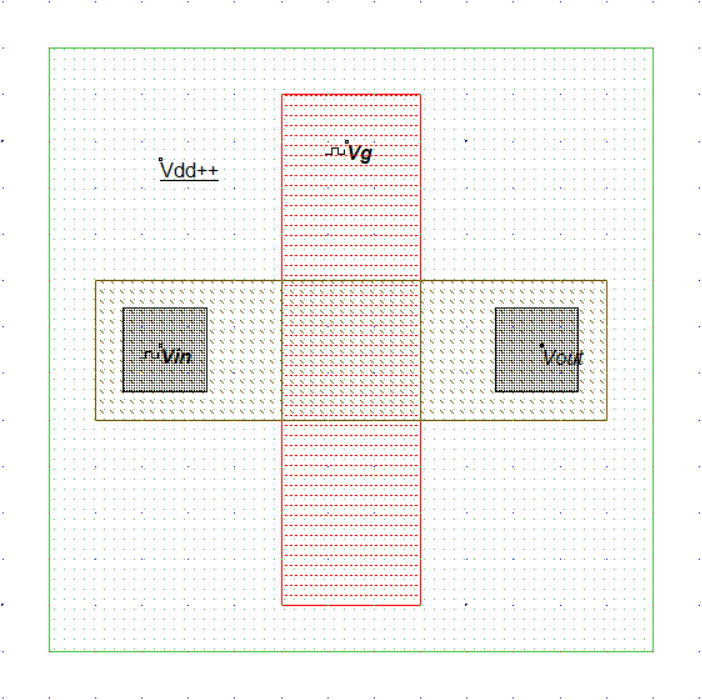
\includegraphics[width=1\textwidth, height=0.25\textheight]{Images/pmos/pimg1.png}
			\caption{pMOS}
			\label{fig:3-b}
		\end{subfigure}
		\hfill
		\begin{subfigure}[t]{0.49\textwidth}
			\centering
			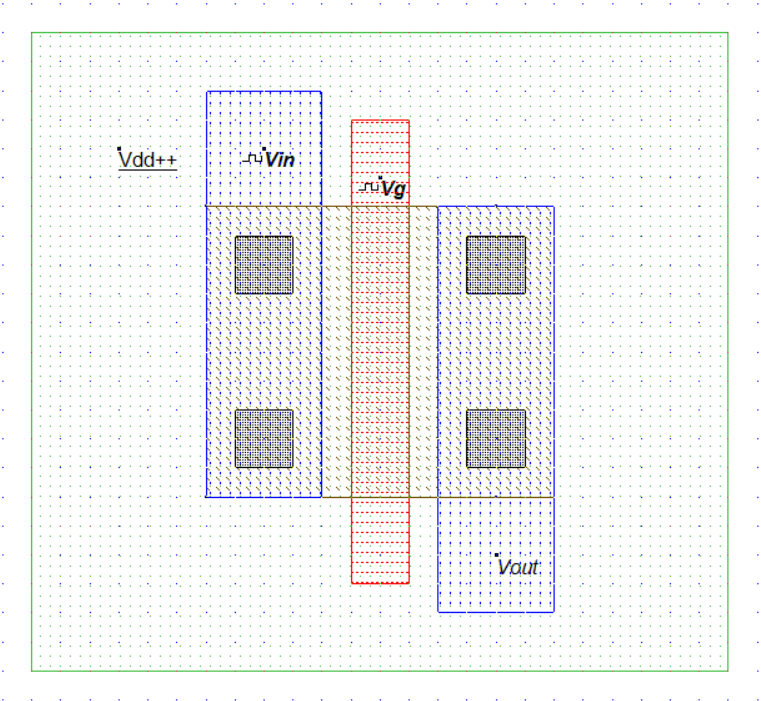
\includegraphics[width=1\textwidth, height=0.25\textheight]{Images/Builtin pmos/pmos2.png}
			\caption{pMOS (using MOS GENERATOR)}
			\label{fig:3-b}
		\end{subfigure}
		\caption{  Design of nMos and pMos layout ensuring proper DRC.}
		\label{fig:1}
	\end{figure}
	
	
	
	\clearpage
	
	
	
	\section{Specification}
	
	\subsection{nMOS and pMOS}
	
	\begin{figure}[H]
		\centering
		\begin{subfigure}[t]{0.49\textwidth}
			\centering
			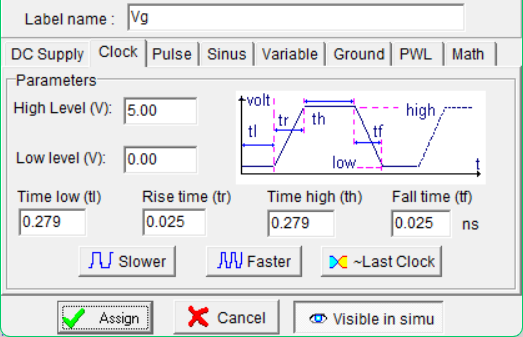
\includegraphics[width=.75\textwidth , height=.15\textheight]{Images/nmos/nspec1.png}
			\caption{Vg for nMOS}
			\label{fig:3-a}
		\end{subfigure}
		\hfill
		\begin{subfigure}[t]{0.49\textwidth}
			\centering
			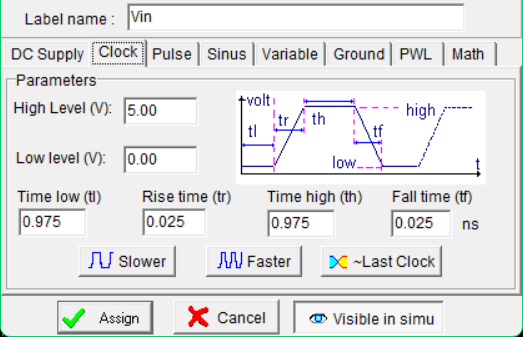
\includegraphics[width=.75\textwidth, height=0.15\textheight]{Images/nmos/nspec2.1.png}
			\caption{Vin for nMOS}
			\label{fig:3-b}
		\end{subfigure}
		
		\vspace{1em}
		
		\begin{subfigure}[t]{0.32\textwidth}
			\centering
			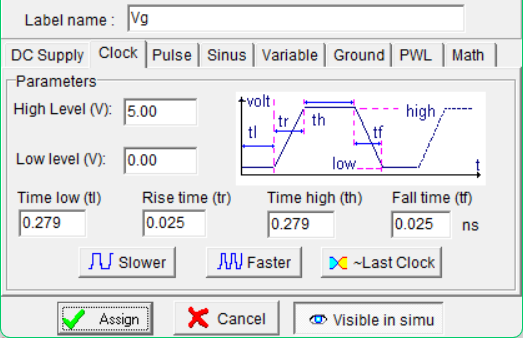
\includegraphics[width=1\textwidth, height=0.13\textheight]{Images/pmos/pspec1.2.png}
			\caption{Vg for pMOS}
			\label{fig:3-c}
		\end{subfigure}
		\hfill
		\begin{subfigure}[t]{0.32\textwidth}
			\centering
			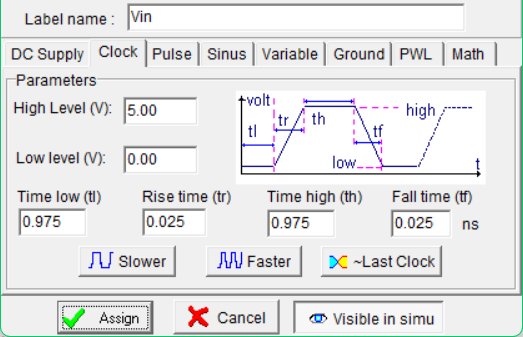
\includegraphics[width=1\textwidth, height=0.13\textheight]{Images/pmos/pspec2.2.png}
			\caption{Vin for pMOS}
			\label{fig:3-d}
		\end{subfigure}
		\hfill
		\begin{subfigure}[t]{0.32\textwidth}
			\centering
			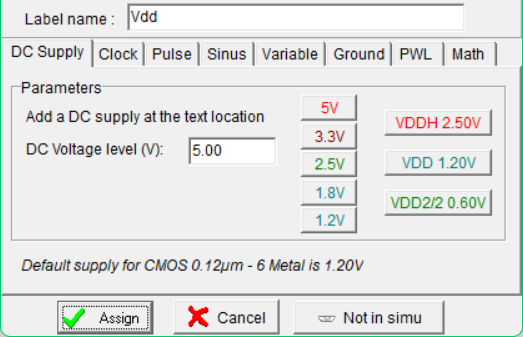
\includegraphics[width=1\textwidth, height=0.13\textheight]{Images/pmos/pspec4.png}
			\caption{Vdd for pMOS}
			\label{fig:3-e}
		\end{subfigure}
		
		\caption{Specifications of nMOS and pMOS layout}
		\label{fig:1}
	\end{figure}
	
	\subsection{nMOS and pMOS using MOS Generator}
	
	\begin{figure}[H]
		\centering
		\begin{subfigure}[t]{0.49\textwidth}
			\centering
			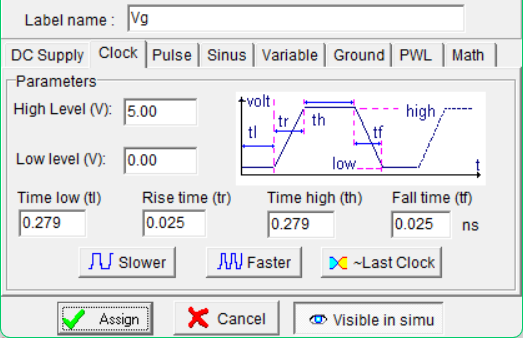
\includegraphics[width=.75\textwidth , height=.15\textheight]{Images/Builtin nmos/nspec4.png}
			\caption{Vg for nMOS (using MOS Generator)}
			\label{fig:3-f}
		\end{subfigure}
		\hfill
		\begin{subfigure}[t]{0.49\textwidth}
			\centering
			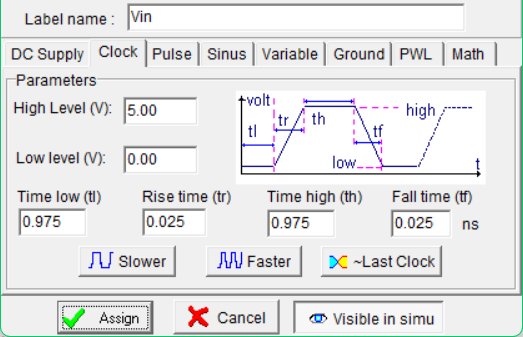
\includegraphics[width=.75\textwidth, height=0.15\textheight]{Images/Builtin nmos/nspec5.png}
			\caption{Vin for nMOS (using MOS Generator)}
			\label{fig:3-g}
		\end{subfigure}
		
		\vspace{1em}
		
		\begin{subfigure}[t]{0.32\textwidth}
			\centering
			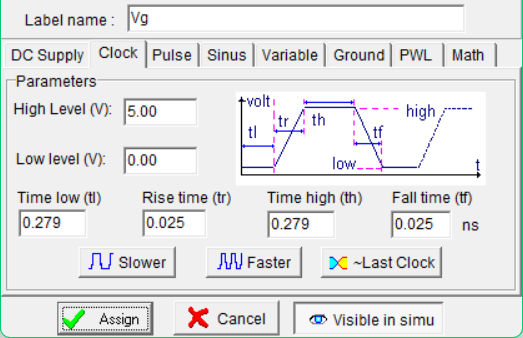
\includegraphics[width=1\textwidth, height=0.13\textheight]{Images/Builtin pmos/pspec4.png}
			\caption{Vg for pMOS (using MOS Generator)}
			\label{fig:3-h}
		\end{subfigure}
		\hfill
		\begin{subfigure}[t]{0.32\textwidth}
			\centering
			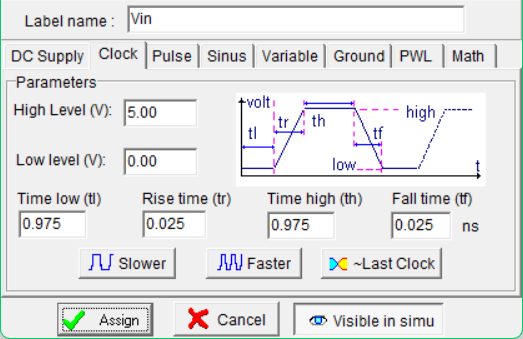
\includegraphics[width=1\textwidth, height=0.13\textheight]{Images/Builtin pmos/pspec5.png}
			\caption{Vin for pMOS (using MOS Generator)}
			\label{fig:3-i}
		\end{subfigure}
		\hfill
		\begin{subfigure}[t]{0.32\textwidth}
			\centering
			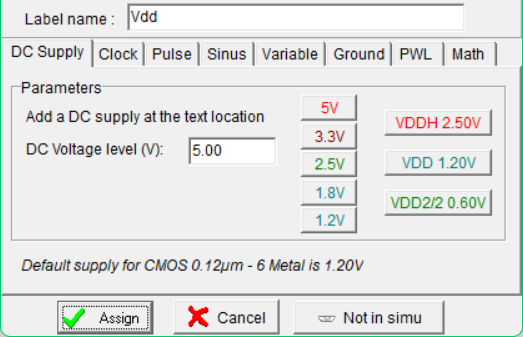
\includegraphics[width=1\textwidth, height=0.13\textheight]{Images/Builtin pmos/pspec6.png}
			\caption{Vdd for pMOS (using MOS Generator)}
			\label{fig:3-j}
		\end{subfigure}
		
		\caption{Specifications of nMOS and pMOS (using MOS Generator)}
		\label{fig:2}
	\end{figure}
	
	
	
	\section{Output Waveshape }
	\subsection{nMOS and pMOS}
	\begin{figure}[H]
		\centering
		\begin{subfigure}[t]{1\textwidth}
			\centering
			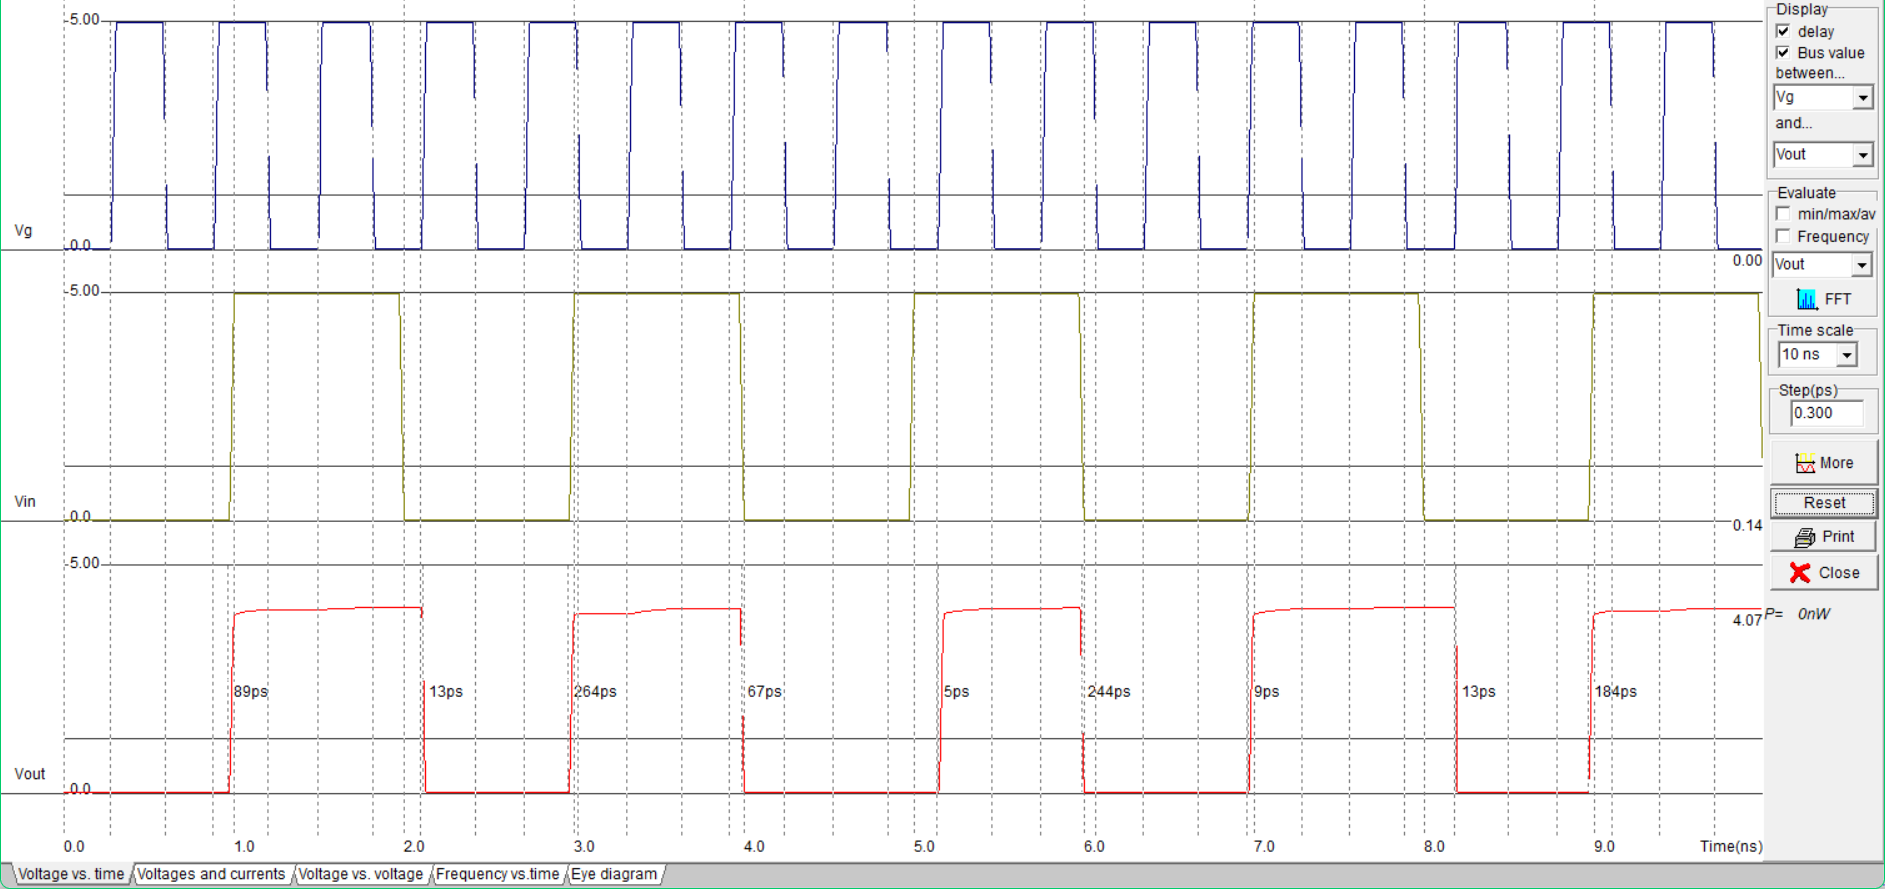
\includegraphics[width=1\linewidth]{Images/nmos/nsim1.png}
			\caption{nMOS}
			\label{fig:enter-label}
		\end{subfigure}
		\\[1cm]
		\begin{subfigure}[t]{1\textwidth}
			\centering
			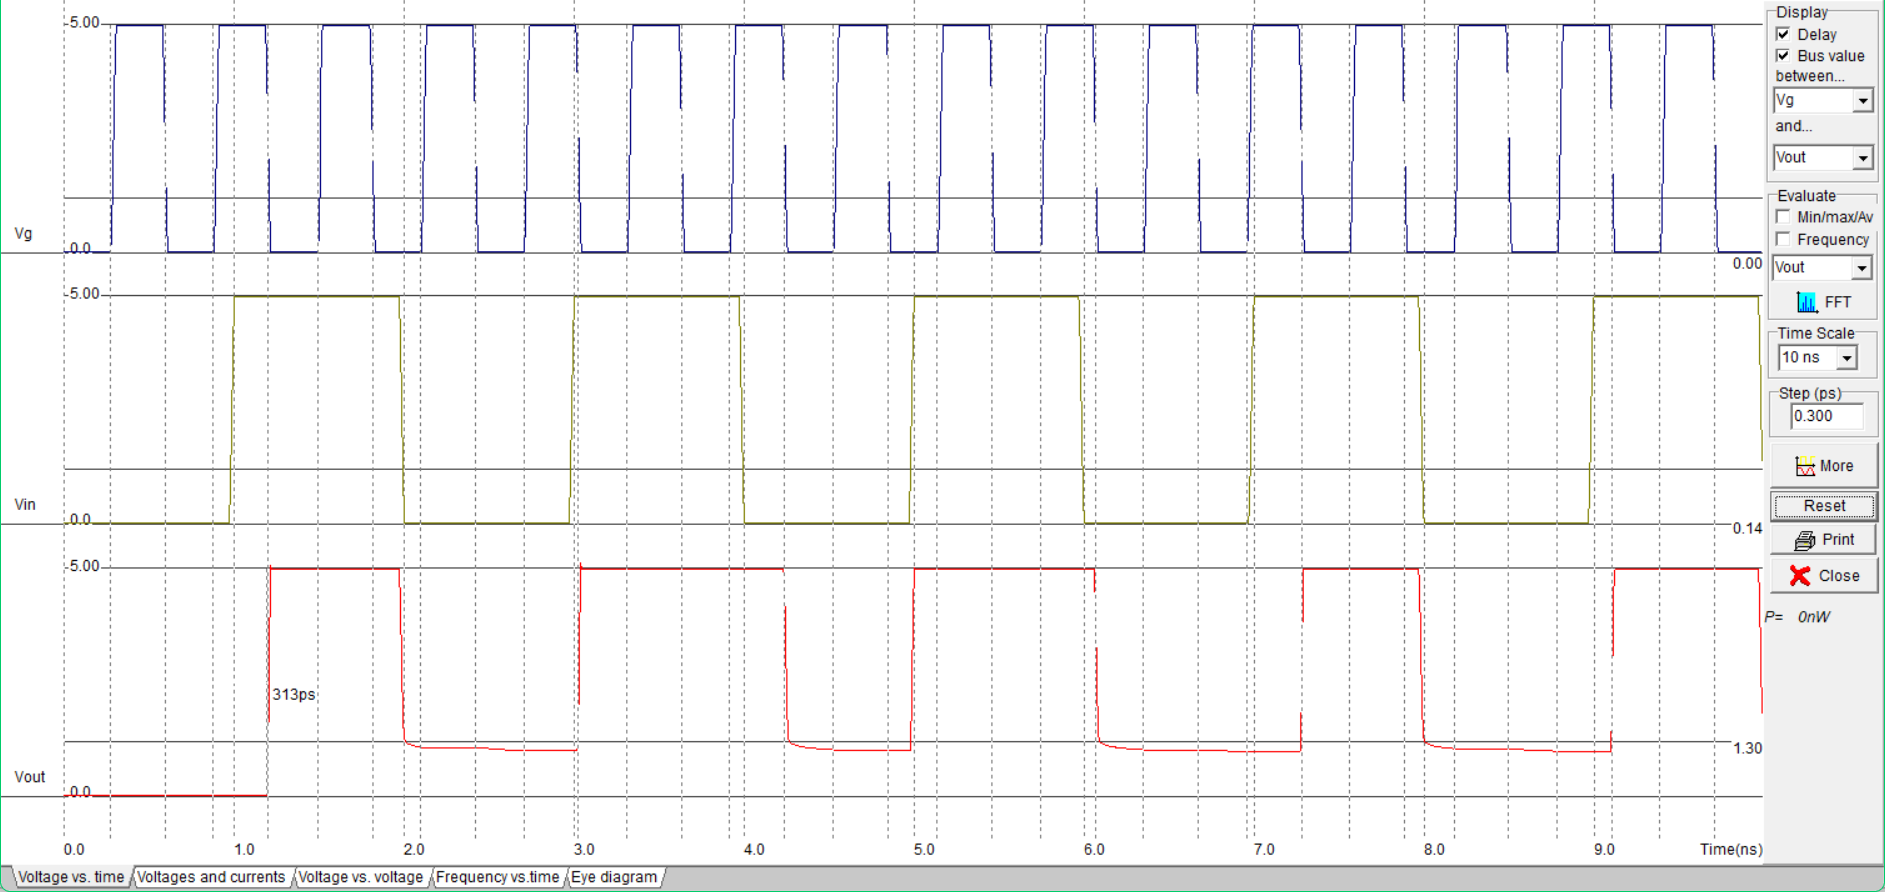
\includegraphics[width=1\linewidth]{Images/pmos/psim1.2.png}
			\caption{pMOS}
			\label{fig:enter-label}
		\end{subfigure}
		\caption{Output Waveshape of Fabricated nMOS and pMOS}
	\end{figure}
	
	\subsection{nMOS and pMOS using MOS Generator}
	\begin{figure}[H]
		\centering
		\begin{subfigure}[t]{1\textwidth}
			\centering
			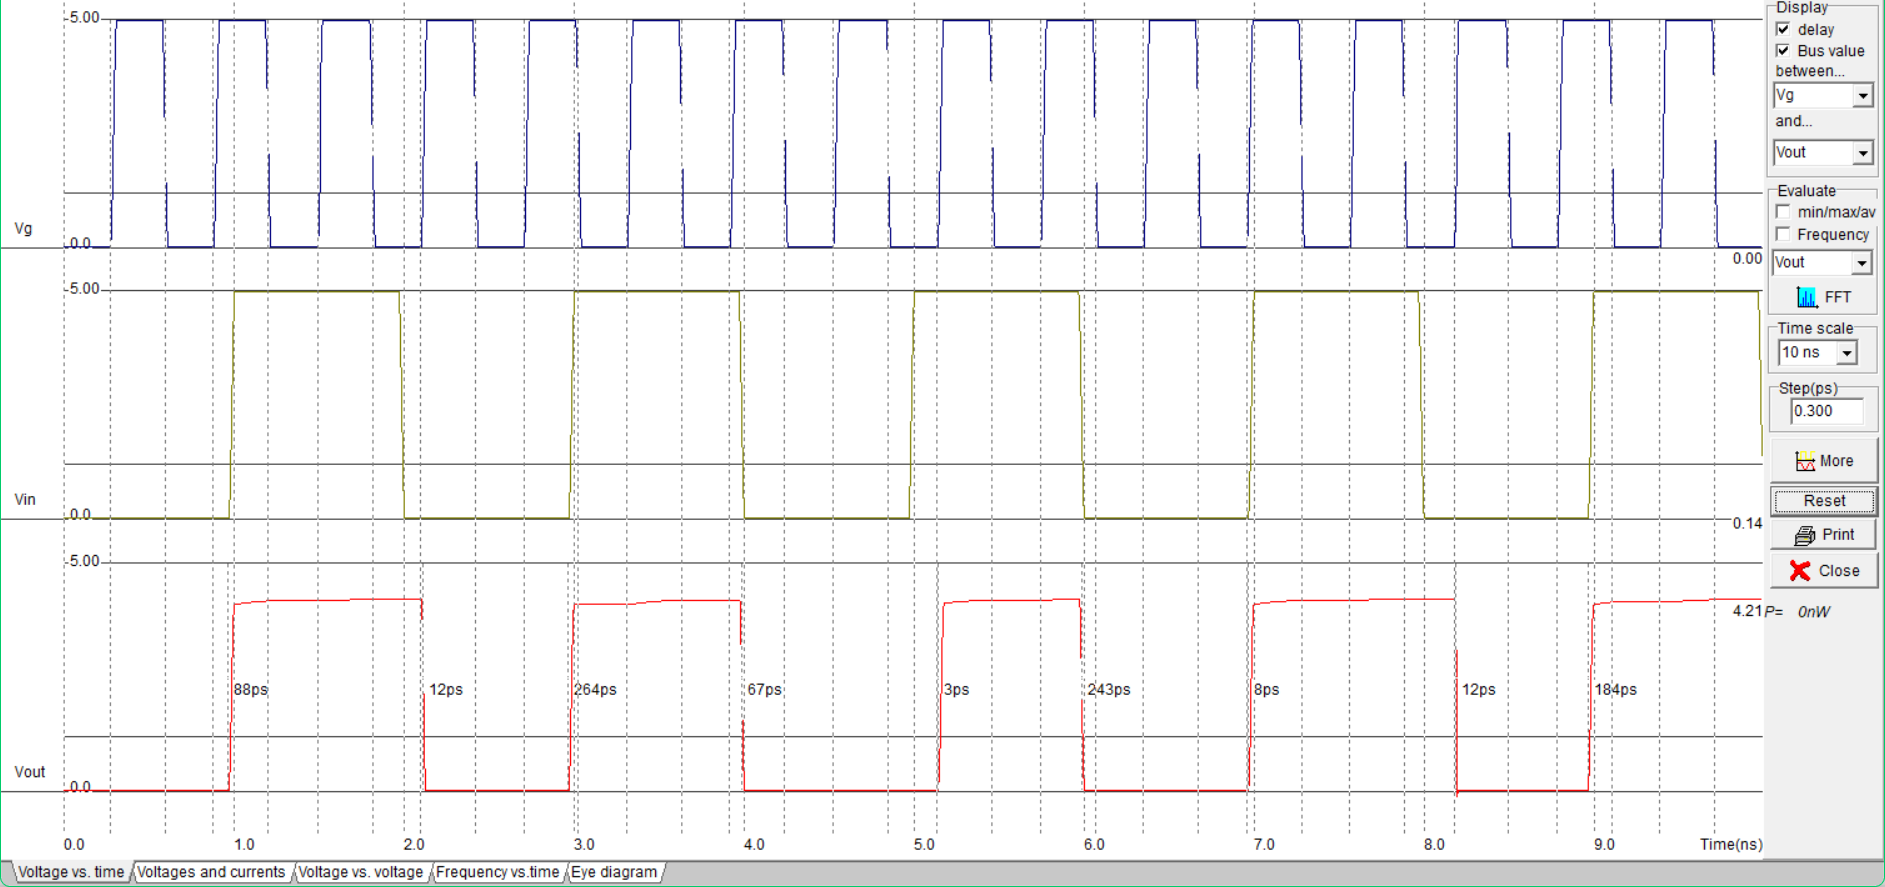
\includegraphics[width=1\linewidth]{Images/Builtin nmos/nsim2.png}
			\caption{nMOS using MOS Generator}
			\label{fig:enter-label}
		\end{subfigure}
		\\[1cm]
		\begin{subfigure}[t]{1\textwidth}
			\centering
			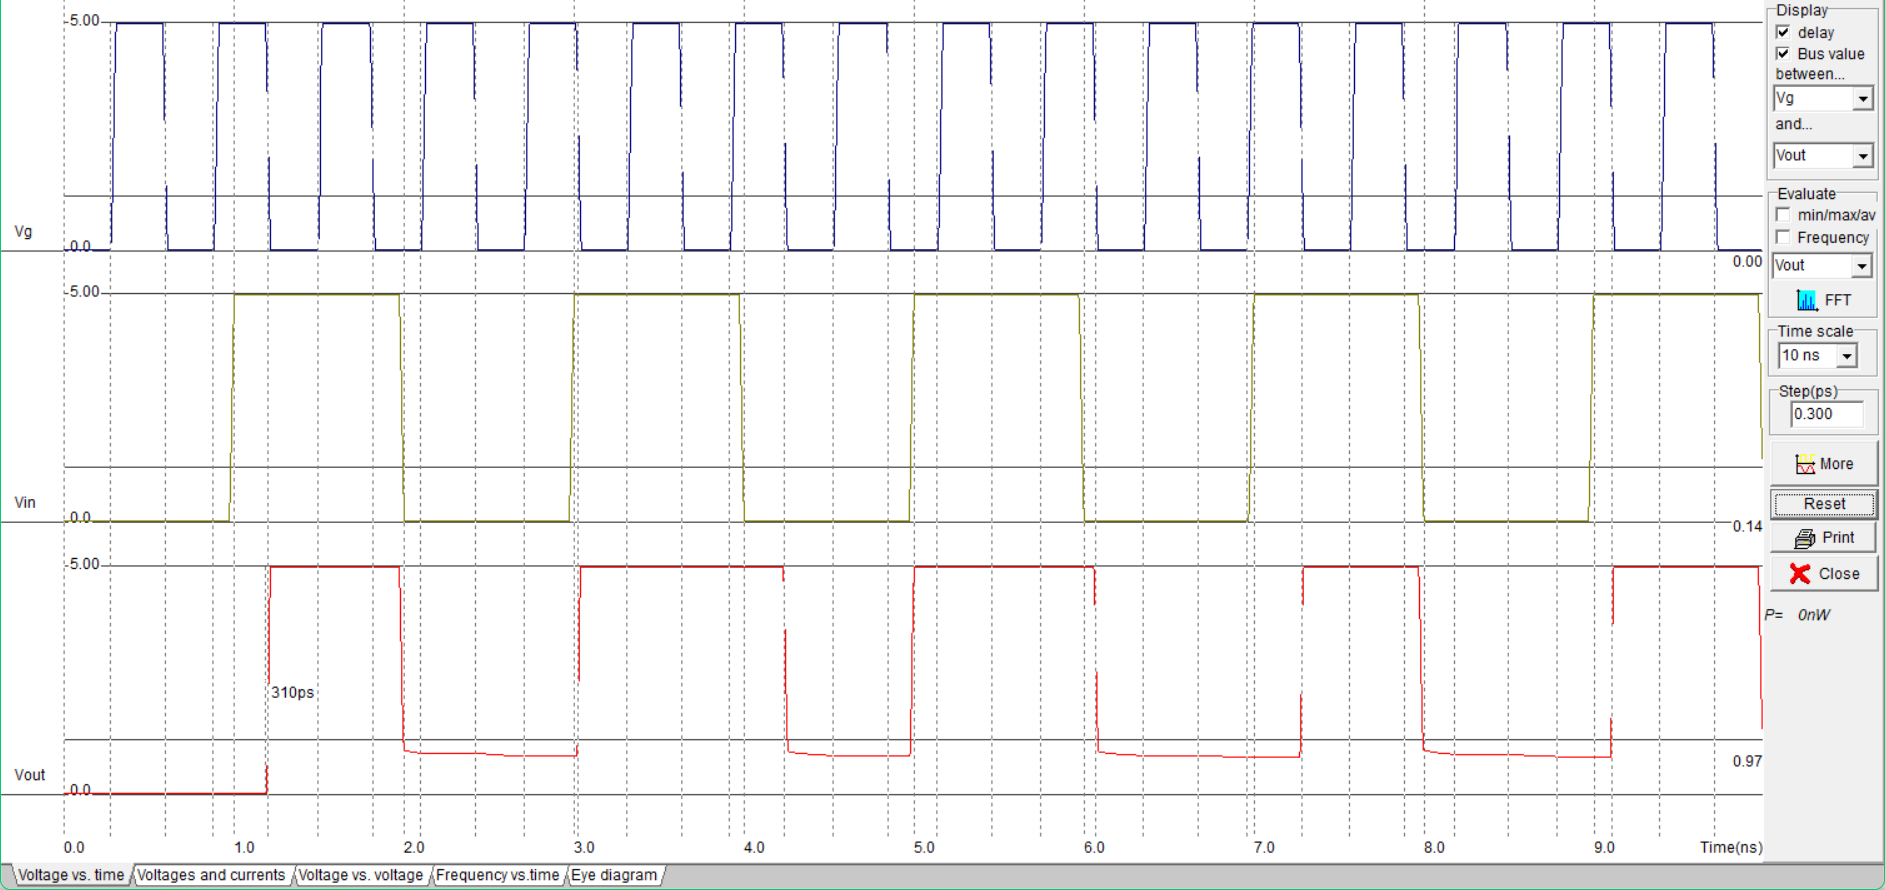
\includegraphics[width=1\linewidth]{Images/Builtin pmos/psim2.png}
			\caption{pMOS using MOS Generator}
			\label{fig:enter-label}
		\end{subfigure}
		\caption{Output Waveshape of nMOS and pMOS (using MOS Generator)}
	\end{figure}
	\newpage
	\section{Discussion }
	In this lab report, we utilized Microwind 3.0 to design and simulate nMOS and pMOS transistors, focusing on both their theoretical understanding and practical fabrication steps. The software's user-friendly interface, featuring a variety of menus such as File, View, Edit, Simulate, Compile, and Analysis, enabled efficient layout creation and simulation of MOS transistors.\\
	
	The nMOS transistor was explored as a "strong 0, poor 1" device, where it conducts well to ground, making it effective for creating strong logical zeros, but less efficient at generating logical ones. Conversely, the pMOS transistor operates as a "strong 1, poor 0" device, excelling at producing strong logical ones, but offering weaker performance when pulling signals to zero.\\
	
	The fabrication of both nMOS and pMOS transistors using Microwind involved defining diffusion layers and polysilicon gates, with the MOS generator providing a streamlined way to create layouts. This allowed us to visualize the physical structure and electrical characteristics of the transistors, and also perform simulations to verify their output voltage based on input voltage and ground voltage.\\
	
	The simulation results confirmed the theoretical expectations regarding the performance of nMOS and pMOS transistors, highlighting their complementary nature in digital logic circuits.
	
\end{document}
